\documentclass{standalone} 

\usepackage{amsmath}
\usepackage{graphicx,tikz}
\usepackage{pgfplots,tikz-3dplot}
\pgfplotsset{compat=1.8}
\usetikzlibrary{shapes.geometric}
\usepgfplotslibrary{fillbetween}
\usetikzlibrary{patterns}

\newcommand{\domain}{D}

\begin{document}

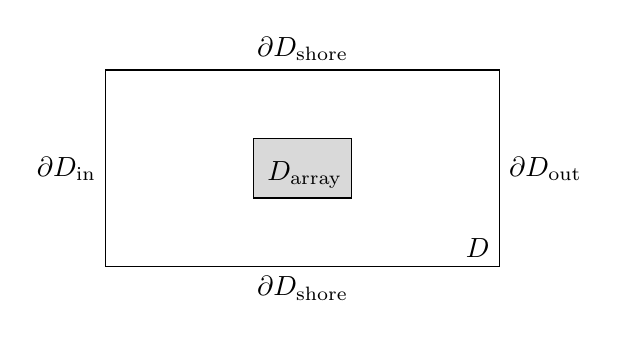
\begin{tikzpicture}[scale=0.25]
	% computational domain
	\draw (0,0) -- (20, 0) -- (20, 10) -- (0, 10) -- cycle;
	\node[above left] at (20,0) {$\domain$};
	% array
	\draw[fill=gray!30] (750/100,350/100) -- (1250/100, 350/100) -- 
	(1250/100, 650/100) -- (750/100, 650/100) -- cycle;
	\node[above left] at (1250/100, 350/100) {$\domain_{\text{array}}$};
	% boundaries
	\node[left] at (0,5) {$\partial D_{\text{in}}$};
	\node[right] at (20,5) {$\partial D_{\text{out}}$};
	\node[below] at (10,0) {$\partial D_{\text{shore}}$};
	\node[above] at (10,10) {$\partial D_{\text{shore}}$};
	% velocity
	%		\draw[->] (0,5) -- (2, 5) node[midway, below]{$y$};
\end{tikzpicture}




\end{document}
